%\documentclass[10pt]{beamer}
\documentclass[handout,10pt]{beamer}
%\usepackage{xeCJK}
\usepackage{ctex}

%\usepackage[orientation=landscape,size=custom,width=16,height=12,scale=0.5,debug]{beamerposter}

 % 1. packages

 % ----------- fonts and symbles ---------
\usepackage{amsmath,amssymb,amsfonts,amsthm}
%\usepackage{CJK}
\usepackage{dsfont}
\usepackage{mathrsfs}
\usepackage{eucal} % for \mathcal

%\renewcommand{\rmdefault}{ptm}


%\usepackage{fontspec}
%\newfontfamily\monaco{Monaco}

%\usepackage{mathbbold} %,bbold

 \usepackage{textcomp} % for \textnormal{\textperthousand}
% -----------------





%\usepackage{slashbox}
%\usepackage[margin=2.2cm]{geometry} % |geometry| package clash with |booktabs| package
%\usepackage{cases}
% -------- tables -------
\usepackage{booktabs} % for \toprule, \bottomrule
\usepackage{tabularx}
\usepackage{multirow}
% --------- figures ---------
\usepackage{graphicx}
% ---------- algorithms -------
\usepackage{algorithm}
\usepackage{algorithmic}
%\usepackage{footnote}
    % |footnote| package occurs error:
    % Runaway argument?
    % \def \insertfootnotetext {\@@ }\def \insertfootnotemark {\@makefnmark \ETC.

\usepackage{listings}

\usepackage[linewidth=1pt]{mdframed} % for  mdframe environment




 \usepackage{color}
 \usepackage{xcolor}     %¸ßÁÁʹÓõÄÑÕÉ«

\usepackage{setspace}
%%\usepackage{type1cm}
\usepackage{adjustbox} % for \adjustbox

\usepackage{accsupp}
\newcommand{\emptyaccsupp}[1]{\BeginAccSupp{ActualText={}}#1\EndAccSupp{}}




%%   figures and tables
\graphicspath{{figure/}}


% 2. new commands

% 2.0 common commands
%\newcommand{\bc}{\begin{center}}
%\newcommand{\ec}{\end{center}}
%\newcommand{\ba}{\begin{array}}
%\newcommand{\ea}{\end{array}}
%\newcommand{\be}{\begin{equation}}
%\newcommand{\ee}{\end{equation}}

% 2.1 colors
\definecolor{dgrey}{rgb}{0.30,0.30,0.30}
\definecolor{lred}{rgb}{0.50,0.00,0.50}
\definecolor{lblue}{rgb}{0.8,0.8,1}
\definecolor{dred}{rgb}{0.6,0,0}
\definecolor{dblue}{rgb}{0,0,0.5}
\definecolor{dgrey}{rgb}{0.35,0.35,0.35}
\definecolor{rred}{rgb}{0.9,0,0}
\definecolor{mylblue}{rgb}{0.3,0.2, 0.8}

\definecolor{commentcolor}{RGB}{85,139,78}
\definecolor{stringcolor}{RGB}{206,145,108}
\definecolor{keywordcolor}{RGB}{34,34,250}
\definecolor{backcolor}{RGB}{220,220,220}

\newcommand{\blue}[1]{{\color{blue}#1}}
\newcommand{\dblue}[1]{{\color{dblue}#1} }
\newcommand{\red}[1]{{\color{red}#1}}
\newcommand{\dred}[1]{{\color{dred}#1}}
\newcommand{\cyan}[1]{{\color{cyan}#1}}
\newcommand{\bfblue}[1]{\textbf{\color{dblue}#1} }
\newcommand{\bfred}[1]{\textbf{\color{dred}#1} }
\newcommand{\green}[1]{{\color{green}#1}}
%\newcommand{\alert}[1]{{\color{red}#1}}
\newcommand{\black}[1]{{\color{black}#1}}
\newcommand{\light}[1]{{\color{blue}\textbf{#1}}}
\newcommand{\hot}[1]{{\color{dred}#1}}
 \newcommand{\highlight}[1]{ \textbf{\color{mylblue}#1}}
 \newcommand{\important}[1]{{\color{red}#1}} % for highlighting  some words

 \newcommand{\mystar}{\dred{$^{\clubsuit}$ }}
  \newcommand{\doublestar}{\dred{$^{\clubsuit\clubsuit}$ }}

\newcommand{\mynote}[1]{{\footnotesize \color{mylblue}#1}}

 \newcommand{\hint}[1]{{\small \color{mylblue}#1}}
\newcommand{\smallhint}[1]{{\small \color{dgrey}#1}}
\newcommand{\footnotehint}[1]{{\footnotesize \color{dgrey}#1}}
\newcommand{\tinyhint}[1]{{\tiny \color{dgrey}#1}}
\newcommand{\mytitle}[1]{\medskip{\large \textbf{\color{mylblue}#1}}}
\newcommand{\normaltitle}[1]{\medskip{ \textbf{\color{mylblue}#1}}}

%\newcommand{\head}[1]{\textbf{\large\color{blue}#1}}
%\newcommand{\heading}[1]{\textbf{\large\color{blue}#1}}

\newcommand{\myfbox}[2]{ \bigskip \begin{center} \fbox{\parbox{#1}{ #2  }} \end{center}\bigskip }

\newcommand{\myvar}[1]{}
%\newcommand{\mynote}[1]{#1}

% 2.2 mathematical symbols

\newcommand{\drightarrow}{\stackrel{d.}{\rightarrow}}
\newcommand{\prightarrow}{\stackrel{p.}{\rightarrow}}
\newcommand{\bernoulli}{\textnormal{Ber}}
\newcommand{\cov}{\mathsf{Cov}}
\newcommand{\corr}{\mathbf{Corr}}
\newcommand{\regret}{\textnormal{Regret}}
\newcommand{\conv}{\textnormal{conv}}
\newcommand{\dotdiv}{\stackrel{\centerdot}{-}}
\newcommand{\dom}{\textnormal{dom}}
\newcommand{\convergenceinprob}{\stackrel{P}{\rightarrow}}
\newcommand{\convergenceindist}{\rightsquigarrow}
\newcommand{\probability}{\mathbb{P}}
\newcommand{\expectation}{\mathbb{E}}
\newcommand{\epi}{\textnormal{epi}}
\newcommand{\variance}{\mathbb{V}}
\newcommand{\var}[1]{\mathbb{V}(#1)}
\newcommand{\covariance}{\mathsf{Cov}}
\newcommand{\empiricalrisk}[1]{\hat{R}(#1)}
\newcommand{\expectedrisk}[1]{R(#1)}
\newcommand{\mgf}[1]{\psi_{#1}(\lambda)}
\newcommand{\mgfexpansion}[1]{\expectation[e^{\lambda#1}]}
\newcommand{\mgfmultivariate}[1]{\expectation[e^{\lambda^\transpose#1}]}
\newcommand{\transpose}{{\mathsf{T}}}
\newcommand{\real}{\mathbb{R}}
\newcommand{\gaussian}[2]{\mathcal{N}(#1,#2)}
\newcommand{\subGaussian}[1]{\mathsf{subG}(#1)}
\newcommand{\indicator}[1]{\mathbb{I}[#1]}
\newcommand{\x}[1]{x^{(#1)}}
\newcommand{\y}[1]{y^{(#1)}}
\newcommand{\z}[1]{z^{(#1)}}
\newcommand{\feature}{x}
\newcommand{\response}{y}
\newcommand{\supofempiricalprocess}{\|\mathbb{P}_n-\mathbb{P}\|_{\decisionspace}}
\newcommand{\decisionspace}{\mathscr{F}}
\newcommand{\decisionfunction}{f}
\newcommand{\featurespace}{\mathcal{X}}
\newcommand{\classifierestimate}{\widehat{h}}
\newcommand{\classifiertrue}{h^\star}
\newcommand{\classifier}{h}
\newcommand{\hypothesisclass}{\mathcal{H}}
\newcommand{\dataset}{\mathcal{D}}
\newcommand{\defineas}{\stackrel{\textnormal{def}}{=}}
\newcommand{\rademachercomplexity}[1]{\mathsf{Rad}_n\left(#1\right)}
\newcommand{\loss}{\ell}
\newcommand{\composite}{\circ}
\newcommand{\convexhull}{\mathsf{conv}}
\newcommand{\norm}[2][2]{\|#2\|_{#1}}
\newcommand{\shatteringcoefficient}[2]{\mathcal{S}(#1,#2)}
\newcommand{\vcdimension}[1]{\mathsf{VC}\left(#1\right)}
\newcommand{\rank}{\mathsf{rank}}
\newcommand{\innerproduct}[2]{\left\langle #1, #2\right\rangle}
\newcommand{\modelparameter}{\theta}
\newcommand{\ball}[3][]{\mathcal{B}_{{#1}}\left(#2,#3\right)}
\newcommand{\metric}{d}
\newcommand{\coveringnumber}[4][]{N_{{#1}}\left(#2,#3,#4\right)}
\newcommand{\trace}{\textnormal{tr}}
\newcommand{\std}{\textnormal{std}}
\newcommand{\sgn}{\textnormal{sign}}
%\renewcommand{\span}{\textnormal{span}}

 % do not overwrite the existing command \span
 % as it leads to an error of
 %  "Missing # Inserted in Alignment Preamble" for ``align'' environment

\newcommand{\myspan}{\textnormal{span}}

%%%
\newcommand{\rightarrowd}{\stackrel{d}{\rightarrow}}
\newcommand{\rightarrowp}{\stackrel{p}{\rightarrow}}
\newcommand{\defeq}{ \stackrel{\textnormal{def}}{=}}
\newcommand{\proj}{ \textnormal{Proj}}
\newcommand{\dist}{\textnormal{dist}}

\newcommand{\argmax}{\textnormal{argmax}}
\newcommand{\argmin}{\textnormal{argmin}}
\newcommand{\subg}{\textnormal{subG}}


 \newcommand{\bba}{\mathbb{A}}
\newcommand{\bbb}{\mathbb{B}}
\newcommand{\bbc}{\mathbb{C}}
\newcommand{\bbd}{\mathbb{D}}
\newcommand{\bbe}{\mathbb{E}}
\newcommand{\bbf}{\mathbb{F}}
\newcommand{\bbg}{\mathbb{G}}
\newcommand{\bbh}{\mathbb{H}}
\newcommand{\bbi}{\mathbb{I}}
\newcommand{\bbj}{\mathbb{J}}
\newcommand{\bbk}{\mathbb{K}}
\newcommand{\bbl}{\mathbb{L}}
\newcommand{\bbm}{\mathbb{M}}
\newcommand{\bbn}{\mathbb{N}}
\newcommand{\bbo}{\mathbb{O}}
\newcommand{\bbp}{\mathbb{P}}
\newcommand{\bbq}{\mathbb{Q}}
\newcommand{\bbr}{\mathbb{R}}
\newcommand{\bbs}{\mathbb{S}}
\newcommand{\bbt}{\mathbb{T}}
\newcommand{\bbu}{\mathbb{U}}
\newcommand{\bbv}{\mathbb{V}}
\newcommand{\bbw}{\mathbb{W}}
\newcommand{\bbx}{\mathbb{X}}
\newcommand{\bby}{\mathbb{Y}}
\newcommand{\bbz}{\mathbb{Z}}

\newcommand{\bfa}{\mathbf{a}}
\newcommand{\bfb}{\mathbf{b}}
\newcommand{\bfc}{\mathbf{c}}
\newcommand{\bfd}{\mathbf{d}}
\newcommand{\bfe}{\mathbf{e}}
\newcommand{\bff}{\mathbf{f}}
\newcommand{\bfg}{\mathbf{g}}
\newcommand{\bfh}{\mathbf{h}}
\newcommand{\bfi}{\mathbf{i}}
\newcommand{\bfj}{\mathbf{j}}
\newcommand{\bfk}{\mathbf{k}}
\newcommand{\bfl}{\mathbf{l}}
\newcommand{\bfm}{\mathbf{m}}
\newcommand{\bfn}{\mathbf{n}}
\newcommand{\bfo}{\mathbf{o}}
\newcommand{\bfp}{\mathbf{p}}
\newcommand{\bfq}{\mathbf{q}}
\newcommand{\bfr}{\mathbf{r}}
\newcommand{\bfs}{\mathbf{s}}
\newcommand{\bft}{\mathbf{t}}
\newcommand{\bfu}{\mathbf{u}}
\newcommand{\bfv}{\mathbf{v}}
\newcommand{\bfw}{\mathbf{w}}
\newcommand{\bfx}{\mathbf{x}}
\newcommand{\bfy}{\mathbf{y}}
\newcommand{\bfz}{\mathbf{z}}

\newcommand{\bfA}{\mathbf{A}}
\newcommand{\bfB}{\mathbf{B}}
\newcommand{\bfC}{\mathbf{C}}
\newcommand{\bfD}{\mathbf{D}}
\newcommand{\bfE}{\mathbf{E}}
\newcommand{\bfF}{\mathbf{F}}
\newcommand{\bfG}{\mathbf{G}}
\newcommand{\bfH}{\mathbf{H}}
\newcommand{\bfI}{\mathbf{I}}
\newcommand{\bfJ}{\mathbf{J}}
\newcommand{\bfK}{\mathbf{K}}
\newcommand{\bfL}{\mathbf{L}}
\newcommand{\bfM}{\mathbf{M}}
\newcommand{\bfN}{\mathbf{N}}
\newcommand{\bfO}{\mathbf{O}}
\newcommand{\bfP}{\mathbf{P}}
\newcommand{\bfQ}{\mathbf{Q}}
\newcommand{\bfR}{\mathbf{R}}
\newcommand{\bfS}{\mathbf{S}}
\newcommand{\bfT}{\mathbf{T}}
\newcommand{\bfU}{\mathbf{U}}
\newcommand{\bfV}{\mathbf{V}}
\newcommand{\bfW}{\mathbf{W}}
\newcommand{\bfX}{\mathbf{X}}
\newcommand{\bfY}{\mathbf{Y}}
\newcommand{\bfZ}{\mathbf{Z}}


\newcommand{\bfSigma}{\mathbf{\Sigma}}
\newcommand{\bfrho}{\mathbf{\rho}}

\newcommand{\cala}{\mathcal{A}}
\newcommand{\calb}{\mathcal{B}}
\newcommand{\calc}{\mathcal{C}}
\newcommand{\cald}{\mathcal{D}}
\newcommand{\cale}{\mathcal{E}}
\newcommand{\calf}{\mathcal{F}}
\newcommand{\calg}{\mathcal{G}}
\newcommand{\calh}{\mathcal{H}}
\newcommand{\cali}{\mathcal{I}}
\newcommand{\calj}{\mathcal{J}}
\newcommand{\calk}{\mathcal{K}}
\newcommand{\call}{\mathcal{L}}
\newcommand{\calm}{\mathcal{M}}
\newcommand{\caln}{\mathcal{N}}
\newcommand{\calo}{\mathcal{O}}
\newcommand{\calp}{\mathcal{P}}
\newcommand{\calq}{\mathcal{Q}}
\newcommand{\calr}{\mathcal{R}}
\newcommand{\cals}{\mathcal{S}}
\newcommand{\calt}{\mathcal{T}}
\newcommand{\calu}{\mathcal{U}}
\newcommand{\calv}{\mathcal{V}}
\newcommand{\calw}{\mathcal{W}}
\newcommand{\calx}{\mathcal{X}}
\newcommand{\caly}{\mathcal{Y}}
\newcommand{\calz}{\mathcal{Z}}


% 3. theorem and environments

%\newtheorem{theorem}{Theorem}%[section]
\newtheorem{proposition}{Proposition}%[section]
%\newtheorem{property}{Property}%[section]
%\newtheorem{lemma}{Lemma}%[section]
%\newtheorem{corollary}{Corollary}%[section]
%\newtheorem{definition}{Definition}%[section]
%\newtheorem{example}{Example}%[section]
%\newtheorem{remark}{Remark}%[section]
%\newtheorem{note}{Note}%[section]
%\newtheorem{problem}{Problem}%[section]
\newtheorem{exercise}{Exercise}
%\newtheorem{assumption}{Assumption}
\newtheorem*{lemma_star}{Lemma}
\newtheorem*{theorem_star}{Theorem}

%\newenvironment{summary}[1][Summary]{\par\medskip   \color{dred}\textbf{\large#1. } }{ \medskip}
%\newenvironment{remark}[1][Remark]{\par\medskip  \begin{small} \color{dblue}\textbf{#1. } }{ \end{small}\medskip}
%\renewenvironment{proof}[1][Proof]{\noindent\textbf{#1.} }{\mbox{} \hfill{\small\textrm{$\Box$}}\vspace{1ex}}
% \newenvironment{answer}[1][Answer]{\par\medskip \color{dblue}\textbf{\large#1. }}{ \medskip}

\newenvironment{summary}[1][总结]{\par\medskip   \color{dred}\textbf{\large#1 } }{ \medskip}
\newenvironment{remark}[1][注意]{\par\medskip   \color{dblue}\textbf{\large#1 } }{ \medskip}
\newenvironment{footnoteremark}{ \color{dblue}\begin{footnotesize} }{\end{footnotesize}}
\renewenvironment{proof}[1][证明]{\noindent\textbf{#1.} }{\mbox{} \hfill{\small\textrm{$\Box$}}\vspace{1ex}}
 \newenvironment{question}[1][Q.]{\par\medskip {\color{lred}\large#1}}{ \medskip}
 \newenvironment{answer}[1][Answer]{\par\medskip \color{dblue}\textbf{\large#1 }}{ \medskip}

% 4. beamer setting




%\newtheorem{definition}{\textbf{¶¨Òå}}[section]
%\newtheorem{proposition}[definition] { \textbf{ÃüÌâ}}
%\newtheorem{lemma}[definition] { \textbf{ÒýÀí}}
%\newtheorem{theorem}[definition]{ \textbf{¶¨Àí}}
%\newtheorem{corollary}[definition] { \textbf{ÍÆÂÛ}}
%\newtheorem{remark}[definition] { \textbf{×¢}}
%\newtheorem{example}[definition] { \textbf{Àý}}

%\newcommand{\shadow}[1]{\begin{center}
%\bf{\textcolor{dblue}{\shadowbox{\parbox{3.8in}
% {\textcolor{red}
% {\vspace{1mm}#1}}}}}
%\end{center}}
%
%\newcommand{\head}[1]{\begin{center}
%\bf{\textcolor{dblue}{\shadowbox{\parbox{3.8in}
% {\textcolor{dred}
% {\vspace{1mm}#1}}}}}
%\end{center}}
%
%
%\newcommand{\heading}[1]{%
%  \begin{center}
%    \large\bf
%    \shadowbox{#1}%
%  \end{center}
%\vspace{1ex minus 1ex}}

% set  space above and below math equations in display style

\expandafter\def\expandafter\normalsize\expandafter{%
    \normalsize
    \setlength\abovedisplayskip{1.5ex}
    \setlength\belowdisplayskip{1.2ex}
    \setlength\abovedisplayshortskip{0.5ex}
    \setlength\belowdisplayshortskip{0.5ex}
}

% Ìí¼ÓÒ³Âë´úÂ룬¹È¸èÕÒµ½µÄ¡£
\addtobeamertemplate{navigation symbols}{}{%
    %\usebeamerfont{footline}%
    %\usebeamercolor[fg]{footline}%
    \setbeamercolor{footline}{fg=blue}
    \setbeamerfont{footline}{series=\bfseries}
    \hspace{1em}%
    \normalsize{\insertframenumber/\inserttotalframenumber}
}

% section numbering
\setbeamertemplate{section in toc}[sections numbered]
\setbeamertemplate{subsection in toc}[subsections numbered]



\lstset{                        %¸ßÁÁ´úÂëÉèÖÃ
%basicstyle=\small, % print whole listing small
%basicstyle=\footnotesize\sffamily, % print whole listing small
basicstyle=\footnotesize\rmfamily, % print whole listing small
%basicstyle=\rmfamily, % print whole listing small
    language=python,                    %PythonÓï·¨¸ßÁÁ
    %linewidth=0.9\linewidth,            %Áбílist¿í¶È
    %basicstyle=\ttfamily,              %ttÎÞ·¨ÏÔʾ¿Õ¸ñ
    commentstyle=\color{commentcolor},  %×¢ÊÍÑÕÉ«
    keywordstyle=\color{keywordcolor},  %¹Ø¼ü´ÊÑÕÉ«
    stringstyle=\color{stringcolor},    %×Ö·û´®ÑÕÉ«
    %showspaces=true,                   %ÏÔʾ¿Õ¸ñ
    numbers=left,                       %ÐÐÊýÏÔʾÔÚ×ó²à
    %numberstyle=\tiny\emptyaccsupp,     %ÐÐÊýÊý×Ö¸ñʽ
    numberstyle=\tiny,                  %ÐÐÊýÊý×Ö¸ñʽ
    numbersep=5pt,                      %Êý×Ö¼ä¸ô
    frame=single,                       %¼Ó¿ò
    framerule=0pt,                      %²»»®Ïß
    %escapeinside=@@,                    %ÌÓÒݱêÖ¾
    escapeinside=``,                    %ÌÓÒݱêÖ¾
    emptylines=1,                       %
    xleftmargin=3em,                    %list×ó±ß¾à
    backgroundcolor=\color{backcolor},  %ÁÐ±í±³¾°É«
    tabsize=4,                          %ÖƱí·û³¤¶ÈΪ4¸ö×Ö·û
    %gobble=4                            %ºöÂÔÿÐдúÂëÇ°4¸ö×Ö·û
    breaklines=true,
    extendedchars=false
    }

\lstdefinestyle{numbers}{numbers=left, stepnumber=1, numberstyle=\tiny, numbersep=10pt}
 \lstdefinestyle{nonumbers}{numbers=none}

\newcommand{\alertcode}[1]{{\color{red}#1}} % used for alerting codes

%\lstset{numbers=left, numberstyle=\tiny,
%keywordstyle=\color{blue!70},
%commentstyle=\color{red!50!green!50!blue!50},
%frame=shadowbox,
%rulesepcolor=\color{red!20!green!20!blue!20},
%escapeinside=``,
%framesep = 2ex,
%rulesep = 1ex
%%framexrightmargin= 1em %
%}


% Vary the color applet  (try out your own if you like)
\colorlet{structure}{red!65!black}

%\beamertemplateshadingbackground{yellow!50}{white}


%\setbeamerfont{normal text}{family=\rmfamily}
%\setbeamerfont{frametitle}{family=\rmfamily}

% Changing the fonts: this will make the slides more readable and the math look like regular tex math
\usefonttheme{serif}



% set spaces

\setstretch{1.2}  % ÉèÖÃÐоà

\addtobeamertemplate{block begin}{\setlength\abovedisplayskip{0pt}} % reduce the large space before a block

% set section number styles



\newcommand{\secno}{Sec.\,\thesection\ }
\newcommand{\subsecno}{Sec.\,\thesubsection\ }

% set logo

 \pgfdeclareimage[width=1.0]{small-logo}{SMaLL.jpg}
%
 \logo{\vbox{\vskip0.1 \hbox{\pgfuseimage{small-logo}}}}

% set math equation fontsize

 \makeatletter
\DeclareMathSizes{\f@size}{10}{5}{5}
\makeatother

% for chinese section name
\hypersetup{CJKbookmarks=true}


%\usepackage{hyperref}
%\hypersetup{hidelinks,
	%	colorlinks=true,
	%	allcolors=black,
	%	pdfstartview=Fit,
	%	breaklinks=true}

% set font size of the math equations
\makeatletter
\DeclareMathSizes{\f@size}{10}{5}{5}
\makeatother

\begin{document}
	%\begin{CJK*}{GBK}{song}
	\lstdefinestyle{numbers}{numbers=left, stepnumber=1, numberstyle=\tiny, numbersep=10pt}
	\lstdefinestyle{nonumbers}{numbers=none}
	
	\addtobeamertemplate{block begin}{\setlength\abovedisplayskip{0pt}}
	
	\setbeamertemplate{itemize items}{\color{black}$\bullet$}
	
	\title[梯度投影法]{6.1 梯度投影法}

\bigskip

\author[]{
	\underline{SMaLL} 
}

\institute[CUP]{
	\inst{1}
	中国石油大学(华东)\\
	SMaLL 课题组   \\
	\blue{small.sem.upc.edu.cn}\\
	liangxijunsd@163.com \\ 
	
}

\date[2023]{\small    2023}
	\subject{6.1 梯度投影法}
	
	\frame{\titlepage}
	
	
	
	\AtBeginSection[]{
		%\frame<handout:1>{
			\begin{frame}
				\frametitle{梯度投影法}
				%\tableofcontents[current,currentsubsection]
				%\tableofcontents[hideallsubsections,currentsection]
				\tableofcontents[current,hideallsubsections]
			\end{frame}
			
			%}
	}
	%%===================================================
	\section{1. 基于投影方法的可行方向和步长规则}
	
	\begin{frame}
		\frametitle{基于投影方法的可行方向}
		
		\begin{equation}
			\begin{array}{cl}
				\min_x & f(x) \\
				s.t. & x\in X\\
			\end{array}
		\end{equation}
		其中 $f$: 凸函数, $X\subseteq \bbr^n$: 凸集. 
		
		梯度投影法是一种可行方向法,具有下面的迭代格式: %of the form
		$$
		x^{k+1}=x^{k}+\alpha^{k}\left(\bar{x}^{k}-x^{k}\right)
		$$
		其中
		$$
		\bar{x}^{k}=\left[x^{k}-s^{k} \nabla f\left(x^{k}\right)\right]^{+}
		$$
		
		\begin{itemize}
			\item $[\cdot]^{+}$ 表示在集合$X$上的投影
			\item $\alpha^{k} \in(0,1]$ 是步长
			\item $s^{k}$ 是正数
		\end{itemize}
	\end{frame}
	%---------------------------------------------
	\begin{frame}
		\frametitle{基于投影方法的可行方向}
		$s^{k}$: 步长.
		
		
		选择 $\alpha^{k} \equiv 1$
		$\rightarrow$ $x^{k+1}=\bar{x}^{k}$,
		$$
		x^{k+1}=\left[x^{k}-s^{k} \nabla f\left(x^{k}\right)\right]^{+}
		$$
		
		\onslide<2->{
			\begin{figure}
				\centering
				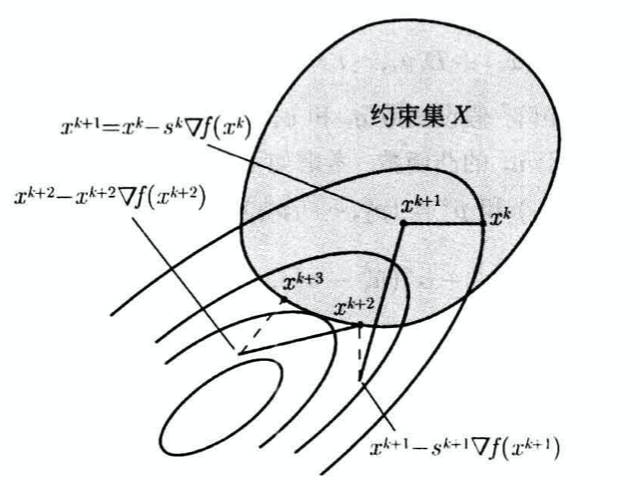
\includegraphics[height=5cm,width=6cm]{picture/gradientProjection.png}
			\end{figure}
		}
	\end{frame}
	%----------------------------------------------
	\begin{frame}
		\frametitle{基于投影方法的可行方向}
		$x^{*}=\left[x^{*}-s \nabla f\left(x^{*}\right)\right]^{+}$, $s>0$ $\leftrightarrow$ $x^{*}$是驻点
		
		\onslide<2->{
			\begin{figure}
				\centering
				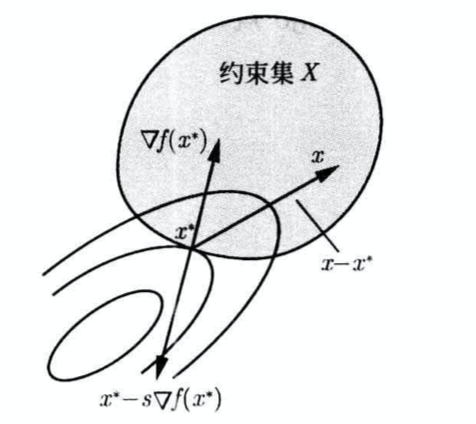
\includegraphics[height=5cm,width=5cm]{picture/stationary-point.png}
			\end{figure}
			
			
			算法停止 $\leftrightarrow$ 遇到驻点时
		}
	\end{frame}
	%----------------------------------------------
	\begin{frame}
		\frametitle{基于投影方法的可行方向}
		如果 $X$ 有相对简单的结构,投影运算通常有显式解
		
		\begin{example}
			当约束集是由上下界限定给出的箱式集合,
			
			$$
			X=\left\{x \mid \alpha_{i} \leq x_{i} \leq \beta_{i}, i=1, \ldots, n\right\}
			$$
			该集合投影向量 $x$的第$i$个分量由下式确定
			
			
			$$
			[x]_{i}^{+}=\left\{\begin{array}{ll}
				\alpha_{i} & \text { 若 } x_{i} \leq \alpha_{i} \\
				\beta_{i} & \text { 若 } x_{i} \geq \beta_{i} \\
				x_{i} & \text { 否则 }
			\end{array}\right.
			$$
		\end{example}
	\end{frame}
	%----------------------------------------------
	\subsection{步长选择和收敛性}
	
	\begin{frame}
		\frametitle{步长选择}
		\begin{itemize}[<+->]
			\item \textbf{固定步长规则}
			
			令$s^{k}$ 为常数 $s>0$
			
			$\alpha^{k}$ 固定为统一值
			$$
			s^{k}=s: \text { 常数 }, \quad \alpha^{k}=1, \quad k=0,1, \ldots
			$$
			
			\item \textbf{缩减步长规则}
			
			$\alpha^{k}$ 为给定常数且
			$$
			s^{k} \rightarrow 0, \quad \sum_{k=0}^{\infty} s^{k}=\infty
			$$
		\end{itemize}
	\end{frame}
	%----------------------------------------------
	\begin{frame}
		\frametitle{步长选择}
		\begin{itemize}
			\item \textbf{有限最小化步长规则}
			
			$s^{k}=s$ :常数 , $k=0,1, \ldots$
			
			$\alpha^{k}$ 取 $[0,1]$且满足
			$$
			f\left(x^{k}+\alpha^{k}\left(\bar{x}^{k}-x^{k}\right)\right)=\min _{\alpha \in[0,1]} f\left(x^{k}+\alpha\left(\bar{x}^{k}-x^{k}\right)\right) .
			$$
			\onslide<2->{
				\item \textbf{沿可行方向的 Armijo 规则}
				
				$s^{k}=s$ : 常数 , $k=0,1, \ldots$
				
				按 Armijo 规则选取$\alpha^{k}$$\in(0,1)$ 
				\begin{itemize}
					\item[-] 对给定的$\beta$和$\sigma$ $\in(0,1)$
					\item[-]取 $\alpha^{k}=\beta^{m_{k}}$, 其中$m_{k}$是使下式成立的第一个非负整数$m$
				\end{itemize}
				$$
				f\left(x^{k}\right)-f\left(x^{k}+\beta^{m}\left(\bar{x}^{k}-x^{k}\right)\right) \geq-\sigma \beta^{m} \nabla f\left(x^{k}\right)^{\prime}\left(\bar{x}^{k}-x^{k}\right)
				$$
			}
		\end{itemize}
	\end{frame}
	%----------------------------------------------
	\begin{frame}
		\frametitle{步长选择}
		\begin{itemize}
			\item \textbf{沿投影弧的 Armijo 规则}
			
			取步长$\alpha^{k}$ 为给定值, 令 $\alpha^{k}=1, \quad k=0,1, \ldots$
			
			$s^{k}$ 逐渐地减小直到 Armijo 不等式成立
			$\rightarrow$
			$$
			\left\{x^{k}(s) \mid s>0\right\}
			$$
			其中
			$$
			x^{k}(s)=\left[x^{k}-s \nabla f\left(x^{k}\right)\right]^{+},s>0
			$$
			\begin{itemize}
				\item[-]选择 $\bar{s}>0, \beta \in(0,1)$, 且 $\sigma \in(0,1)$
				\item[-]设 $s^{k}=\beta^{m_{k}} \bar{s}$,其中 $m_{k}$ 是使
				下面的不等式成立的第一个非负整数$m$
			\end{itemize}
			$$
			f\left(x^{k}\right)-f\left(x^{k}\left(\beta^{m} \bar{s}\right)\right) \geq \sigma \nabla f\left(x^{k}\right)^{\prime}\left(x^{k}-x^{k}\left(\beta^{m} \bar{s}\right)\right)
			$$
		\end{itemize}
	\end{frame}
	%----------------------------------------------
	\subsection{收敛速度}
	\begin{frame}
		\frametitle{收敛速度}
		例如,当目标函数 $f$ 是二次函数
		$$
		f(x)=\frac{1}{2} x^{\prime} Q x-b^{\prime} x,
		$$
		其中 $Q$ 是正定的.
		
		\onslide<2->{
			设 $x^{*}$ 为$X$上$f$的唯一最小解 , 考虑给定步长的情况.
			$$
			\begin{aligned}
				\left\|x^{k+1}-x^{*}\right\| &=\left\|\left[x^{k}-s \nabla f\left(x^{k}\right)\right]^{+}-\left[x^{*}-s \nabla f\left(x^{*}\right)\right]^{+}\right\| \\
				& \leq\left\|\left(x^{k}-s \nabla f\left(x^{k}\right)\right)-\left(x^{*}-s \nabla f\left(x^{*}\right)\right)\right\| \\
				&=\left\|(I-s Q)\left(x^{k}-x^{*}\right)\right\| \\
				& \leq \max \{|1-s m|,|1-s M|\}\left\|x^{k}-x^{*}\right\|
			\end{aligned}
			$$
			其中$m$ 和 $M$ 分别是$Q $的最小和最大的特征值.
		}
	\end{frame}
	%===================================================
	\section{2. 变尺度梯度投影}
	\begin{frame}
		\frametitle{变尺度梯度投影}
		第$k$次迭代, 设$H^{k}$ 是一个正定矩阵,并考虑由
		$$
		x=\left(H^{k}\right)^{-1 / 2} y
		$$
		\onslide<2->{
			那么问题可以写做
			$$
			\begin{array}{l}
				\text{minimize } h^{k}(y) \equiv f\left(\left(H^{k}\right)^{-1 / 2} y\right) \\
				\text {subject to }  y \in Y^{k},
			\end{array}
			$$
			其中 $Y^{k}$ 是集合
			$$
			Y^{k}=\left\{y \mid\left(H^{k}\right)^{-1 / 2} y \in X\right\} .
			$$
		}
	\end{frame}
	%---------------------------------------------------------------
	\begin{frame}
		\frametitle{变尺度梯度投影}
		该问题的梯度投影迭代形式如下
		$$
		y^{k+1}=y^{k}+\alpha^{k}\left(\bar{y}^{k}-y^{k}\right)
		$$
		其中
		$$
		\bar{y}^{k}=\left[y^{k}-s^{k} \nabla h^{k}\left(y^{k}\right)\right]^{+}
		$$
		
		\onslide<2->{
			$\bar{y}^{k}$ 可以定义为使表达式最小化的向量
			$$
			\left\|y-y^{k}+s^{k} \nabla h^{k}\left(y^{k}\right)\right\|^{2}=\left(s^{k}\right)^{2}\left\|\nabla h^{k}\left(y^{k}\right)\right\|^{2}+2 s^{k} \nabla h^{k}\left(y^{k}\right)^{\prime}\left(y-y^{k}\right)+\left\|y-y^{k}\right\|^{2}
			$$
			over $y \in Y^{k}$.
			
		}
	\end{frame}
	%--------------------------------------------------------
	\begin{frame}
		\frametitle{变尺度梯度投影}
		忽略表达式
		$\left(s^{k}\right)^{2}\left\|\nabla h^{k}\left(y^{k}\right)\right\|^{2}$ 并除以$2 s^{k}$,
		$$
		\bar{y}^{k}=\arg \min _{y \in Y^{k}}\left\{\nabla h^{k}\left(y^{k}\right)^{\prime}\left(y-y^{k}\right)+\frac{1}{2 s^{k}}\left\|y-y^{k}\right\|^{2}\right\}
		$$
		
		\onslide<2->{
			通过变化
			$$
			x=\left(H^{k}\right)^{-1 / 2} y, \quad x^{k}=\left(H^{k}\right)^{-1 / 2} y^{k}, \quad \bar{x}^{k}=\left(H^{k}\right)^{-1 / 2} \bar{y}^{k}
			$$
			$$
			\nabla h^{k}\left(y^{k}\right)=\left(H^{k}\right)^{-1 / 2} \nabla f\left(x^{k}\right)
			$$
			迭代可以写成
			$$
			x^{k+1}=x^{k}+\alpha^{k}\left(\bar{x}^{k}-x^{k}\right)
			$$
			其中
			$$
			\bar{x}^{k}=\arg \min _{x \in X}\left\{\nabla f\left(x^{k}\right)^{\prime}\left(x-x^{k}\right)+\frac{1}{2 s^{k}}\left(x-x^{k}\right)^{\prime} H^{k}\left(x-x^{k}\right)\right\}
			$$
		}
	\end{frame}
	%===================================================
	\section{3. 约束牛顿法}
	\begin{frame}
		\frametitle{约束牛顿法}
		$f$ 是二阶连续可微函数.
		
		\onslide<2->{
			考虑变尺度梯度投影方法中的矩阵 $H^{k}=\nabla^{2} f\left(x^{k}\right) ,$
			$$
			x^{k+1}=x^{k}+\alpha^{k}\left(\bar{x}^{k}-x^{k}\right)
			$$
			%where
			$$
			\bar{x}^{k}=\arg \min_{x \in X}\left\{\nabla f\left(x^{k}\right)^{\prime}\left(x-x^{k}\right)+\frac{1}{2 s^{k}}\left(x-x^{k}\right)^{\prime} \nabla^{2} f\left(x^{k}\right)\left(x-x^{k}\right)\right\}
			$$
		}
		
		\onslide<3->{
			$s^{k}=1$ $\rightarrow$  $f$在$x^{k}$ 的二阶泰勒展开 \dred{(约束牛顿法)}
		}
		
		\onslide<4->{
			\hint{梯度投影法}: \footnotehint{$\bar{x}^{k}=\left[x^{k}-s^{k} \nabla f\left(x^{k}\right)\right]^{+}$}
			
			
			\footnotehint{
				$$
				\bar{x}^{k}=\argmin_{x \in X}\left\{\nabla f\left(x^{k}\right)^{\prime}\left(x-x^{k}\right)+\frac{1}{2 s^{k}}\left(x-x^{k}\right)^{\prime}  \hint{I} \left(x-x^{k}\right)\right\}
				$$
			}
			
			
			\dred{$\bar{x}^{k} = \argmin_{x \in X}$  linear approx. of $f$ %at $x_k$
				$+$ proximal term \footnotesize{($\frac{1}{2 s^{k}}||x-x^{k}||^2$)}}
			
		}
		
	\end{frame}
	
	
	
	
	%\end{CJK*}
\end{document}
